 % LuaLaTeX文書; 文字コーAドはUTF-8
 \documentclass[unicode,12pt, A4j]{ltjsarticle}% 'unicode'が必要
 %\usepackage{luatexja}% 日本語したい
 \usepackage{luatexja-fontspec}
 %\usepackage[hiragino-pron]{luatexja-preset}% IPAexフォントしたい(ipaex)
 \usepackage[hiragino-pron,deluxe,expert,bold]{luatexja-preset}
\usepackage{tikz}
\usetikzlibrary{arrows.meta}
 \usepackage[english]{babel}%多言語文書を作成する
 \usepackage{amsmath,amssymb}%標準数式表現を拡大する
 \usepackage{physics}
 \usepackage[subpreambles=true,sort=true]{standalone}
% \renewcommand{\kanjifamilydefault}{\gtdefault}% 既定をゴシック体に
 \usepackage[backend=bibtex,style=phys,articletitle=false,biblabel=brackets,chaptertitle=false,pageranges=false]{biblatex}
 %\usepackage[style=authoryear,backend=bibtex]{biblatex}


 \usepackage{mhchem}
 % あとは欧文の場合と同じ

  \usepackage{caption}
  \usepackage[subrefformat=parens]{subcaption}
\title{東大数学理科後期1995年度}
\author{}
\date{}

\begin{document}
\maketitle

\section{問題1}
パスカル三角形の第$n$行の部分和
\begin{align}
 P_n &= \sum_{k=0}^{n} {}_{n}C_{3k}, \\
 Q_n &= \sum_{k=0}^{n} {}_{n}C_{3k+1},\\
 R_n &= \sum_{k=0}^{n} {}_{n}C_{3k+2}
\end{align}
として数列${P_n}$, ${Q_n}$, ${R_n}$を定義する.ただし,$k > n$のとき${}_{n}C_{k} = 0$とする.
\begin{enumerate}
\item $P_{n+1}$, $Q_{n+1}$, $R_{n+1}$を$P_n$, $Q_n$, $R_n$の式として表せ.
\item 一般項$P_n$, $Q_n$, $R_n$を求めよ.
\item $P_{12}$, $Q_{12}$, $R_{12}$を求めよ.
\end{enumerate}

\begin{figure}[h]
 \centering
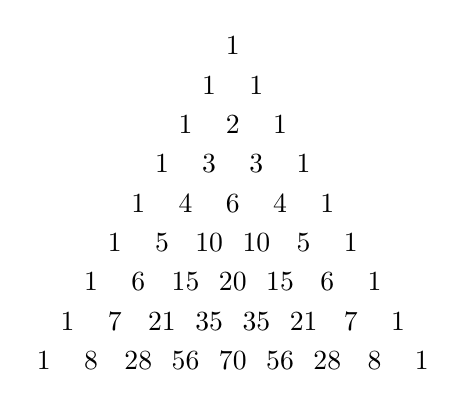
\begin{tikzpicture}
\node at (0,0) {$1$};
\node at (-0.3,-0.5) {$1$};
\node at (0.3,-0.5) {$1$};
\node at (-0.6,-1.0) {$1$};
\node at (0,-1.0) {$2$};
\node at (0.6,-1.0) {$1$};
\node at (-0.9,-1.5) {$1$};
\node at (-0.3,-1.5) {$3$};
\node at (0.3,-1.5) {$3$};
\node at (0.9,-1.5) {$1$};
\node at (-1.2,-2.0) {$1$};
\node at (-0.6,-2.0) {$4$};
\node at (0,-2.0) {$6$};
\node at (0.6,-2.0) {$4$};
\node at (1.2,-2.0) {$1$};
\node at (-1.5,-2.5) {$1$};
\node at (-0.9,-2.5) {$5$};
\node at (-0.3,-2.5) {$10$};
\node at (0.3,-2.5) {$10$};
\node at (0.9,-2.5) {$5$};
\node at (1.5,-2.5) {$1$};
\node at (-1.8,-3.0) {$1$};
\node at (-1.2,-3.0) {$6$};
\node at (-0.6,-3.0) {$15$};
\node at (0,-3.0) {$20$};
\node at (0.6,-3.0) {$15$};
\node at (1.2,-3.0) {$6$};
\node at (1.8,-3.0) {$1$};
\node at (-2.1,-3.5) {$1$};
\node at (-1.5,-3.5) {$7$};
\node at (-0.9,-3.5) {$21$};
\node at (-0.3,-3.5) {$35$};
\node at (0.3,-3.5) {$35$};
\node at (0.9,-3.5) {$21$};
\node at (1.5,-3.5) {$7$};
\node at (2.1,-3.5) {$1$};
\node at (-2.4,-4.0) {$1$};
\node at (-1.8,-4.0) {$8$};
\node at (-1.2,-4.0) {$28$};
\node at (-0.6,-4.0) {$56$};
\node at (0,-4.0) {$70$};
\node at (0.6,-4.0) {$56$};
\node at (1.2,-4.0) {$28$};
\node at (1.8,-4.0) {$8$};
\node at (2.4,-4.0) {$1$};
\end{tikzpicture}
\end{figure}

\section{問題2}
平面上に2点$P$, $Q$があり,$P$と$Q$の距離は1であるとする.このとき,次の(条件)を満たす三角形$ABC$の面積$S$の最大値を求めたい.

(条件) 三角形$ABC$は与えられた平面上にあり,各頂点$A$, $B$, $C$から$P$までの距離または$Q$までの距離のうち,少なくとも一方は1以下である.

\begin{enumerate}
 \item $P$を中心とする半径1の円周を$E$, $Q$を中心とする半径1の円周を$F$とする.上の(条件)の下で最大面積をもつ三角形の頂点$A$, $B$, $C$はそれぞれ$E$または$F$の上にあることを示せ.
 \item この二つの頂点$A$, $B$は円周$E$上にあるとして,この円の中心$P$から弦$AB$におろした垂線の長さを$p$とする.$p$を固定したとき,(条件)を満たす三角形$ABC$の面積$S$が最大となるならば,直線$AB$と直線$PQ$は直交することを示せ.
 \item (条件)を満たす三角形$ABC$の面積$S$の最大値を求めよ.
\end{enumerate}

\section{問題3}
1から13まで,それぞれ違った数字が書かれたカードが1枚ずつ13枚ある.このカードを使って,$A$と$B$の2人が次のルールでゲームをする.
\begin{itemize}
 \item $A$と$B$は最初に2枚ずつカードを持つ.相手のカードの数字は見えない.
 \item まず,$A$が1枚のカードを数字が見えるようにして出し,$B$はそれを見て1枚のカードを出す.数字の大きいカードを出した者が1点を得る.
 \item 次に,残りのカードを出しあって,数字の大きいカードを出した者が1点を得る.
 \item この際,$A$と$B$はおのおのの得点が最大となるようにカードを出すものとする.
\end{itemize}

\begin{enumerate}
 \item カードが配られた後,$A$は手持ちのカードのうち,数字の大きいものを最初に出した方が有利か,不利か,あるいはどちらを出しても同じか.
 \item $A$, $B$に無作為に2枚ずつカードを配った場合,$A$の得る点数の期待値を求めよ.
 \item $A$はカードの数字の合計が14となるような2枚のカードを最初に選んで持っているものとする.$B$は残りのカードから無作為に2枚のカードを選んでゲームを行なう.この場合,$A$ははじめにどのようにカードを選べば$A$の得る点数の期待値が最大となるか,また最小となるか.それぞれの場合の得点の期待値を求めよ.
\end{enumerate}

\end{document}